\section{1174086 - Tia Nur Candida}

\subsection{Teori}
\begin{enumerate}
	\item Jelaskan dengan ilustrasi gambar sendiri apa perbedaan antara vanilla GAN dan cGAN.\\
	Vanilla GANs biasanya tidak memiliki convolutional Neural Jaringan (CNNs) di jaringan mereka.
Conditional GANs (cGANs) adalah perpanjangan dari model GAN. Mereka memungkinkan untuk generasi gambar yang memiliki kondisi tertentu atau atribut dan telah terbukti menjadi lebih baik dari Vanilla GANs sebagai hasilnya. \\
cGANs adalah jenis GAN yang dikondisikan pada beberapa informasi tambahan.  informasi tambahan y ke Generator sebagai lapisan input tambahan. Dalam Vanilla GANs, tidak ada kontrol atas Kategori gambar yang dihasilkan. Ketika kita menambahkan kondisi y ke Generator, kita dapat menghasilkan gambar dari kategori tertentu, menggunakan y, yang mungkin jenis data, seperti label kelas atau data integer. Vanilla GANs bisa belajar hanya satu kategori dan sangat sulit untuk arsitek GANs untuk beberapa kategori. Sebuah cGAN, bagaimanapun, dapat digunakan untuk menghasilkan model multi-modal dengan kondisi yang berbeda untuk kategori yang berbeda.

	\hfill \break
	\begin{figure}[H]
		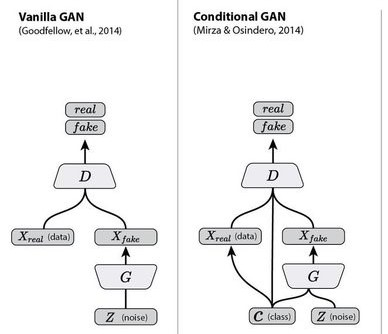
\includegraphics[width=4cm]{figures/1174086/9/1.jpg}
		\centering
		\caption{Illustrasi Vanilla GAN dan cGAN}
	\end{figure}
	\item Jelaskan dengan ilustrasi gambar sendiri arsitektur dari Age-cGAN.
	\hfill \break
	
	Arsitektur cGAN untuk penuaan wajah sedikit lebih rumit. AgecGan terdiri dari empat jaringan: Encoder, FaceNet, Jaringan Generator, dan jaringan diskriminator. Dengan Encoder, kita belajar pemetaan invers gambar wajah masukan dan kondisi usia dengan vektor laten. FaceNet adalah jaringan pengenalan wajah yang mempelajari perbedaan antara gambar input x dan gambar yang direkonstruksi. Kami memiliki jaringan Generator, yang mengambil representasi tersembunyi yang terdiri dari gambar wajah dan vektor kondisi dan menghasilkan gambar. Jaringan diskriminator adalah untuk mendiskriminasikan antara gambar nyata dan gambar palsu. Masalah dengan cGANs adalah bahwa mereka tidak dapat mempelajari tugas pemetaan terbalik masukan gambar x dengan atribut y ke vektor laten z. Solusi untuk masalah ini adalah dengan menggunakan jaringan Encoder. Kita dapat melatih jaringan encoder untuk memperkirakan pemetaan terbalik dari input Images x. 
	\begin{figure}[H]
    	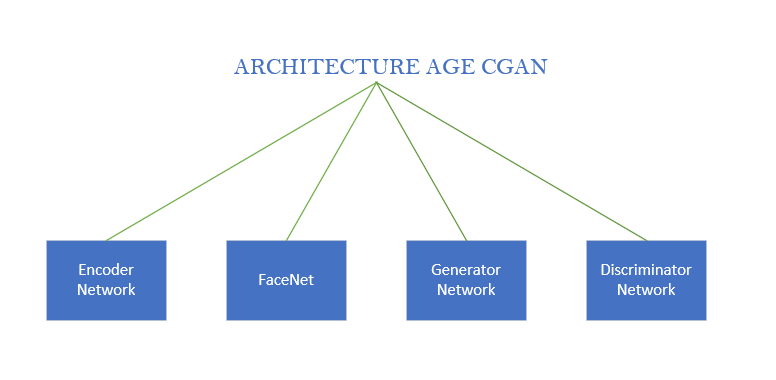
\includegraphics[width=4cm]{figures/1174086/9/2.PNG}
    	\centering
    	\caption{Illustrasi Arsitektur cGAN}
	\end{figure}
	\item Jelaskan dengan ilustrasi gambar sendiri arsitektur encoder network dari AgecGAN.
	\hfill \break
	Tujuan utama dari jaringan Encoder adalah untuk menghasilkan vektor laten dari gambar yang disediakan. Pada dasarnya, dibutuhkan gambar dimensi (64, 64, 3) dan mengubahnya menjadi vektor 100-dimensi. Jaringan Encoder adalah jaringan syaraf convolutional yang dalam. Jaringan berisi empat convolutional blok dan dua lapisan padat. Setiap blok convolutional berisi lapisan convolutional, lapisan normalisasi batch, dan fungsi aktivasi. Di setiap blok convolutional, setiap lapisan convolutional diikuti oleh lapisan normalisasi batch, kecuali lapisan convolutional pertama. 
	\begin{figure}[H]
		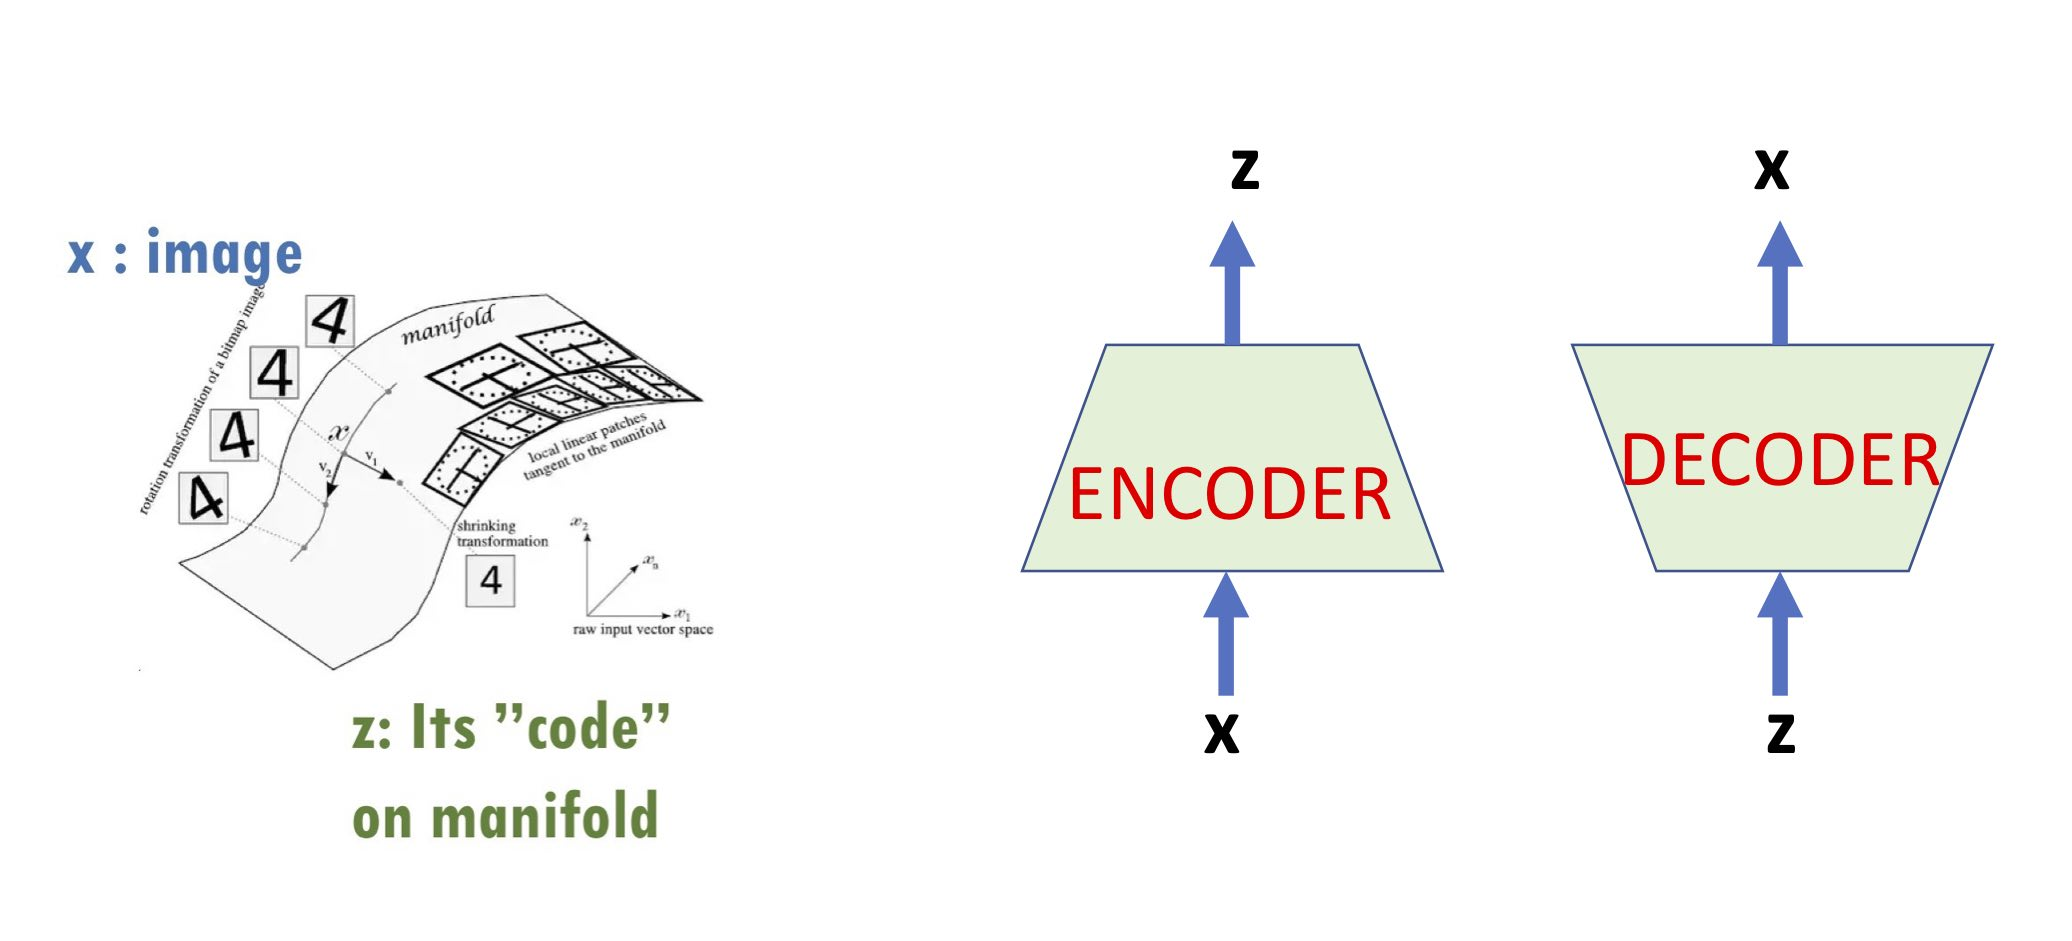
\includegraphics[width=4cm]{figures/1174086/9/3.jpg}
		\centering
		\caption{Illustrasi Network Encoder}
	\end{figure}
	\item Jelaskan dengan ilustrasi gambar sendiri arsitektur generator network dari AgecGAN.
	\hfill \break
	Tujuan utama dari generator adalah untuk menghasilkan gambar dari dimensi (64, 64, 3). Dibutuhkan vektor laten 100 dimensi dan beberapa informasi tambahan, y, dan mencoba untuk menghasilkan gambar yang realistis. Jaringan Generator adalah jaringan neural yang mendalam convolutional juga. Hal ini terdiri dari lapisan padat, upsampling, dan convolutional. Dibutuhkan dua nilai input: vektor kebisingan dan nilai pengkondisian. Nilai pengkondisian adalah informasi tambahan yang diberikan ke jaringan. Untuk Age-cGAN, ini akan menjadi usia. 
	\begin{figure}[H]
		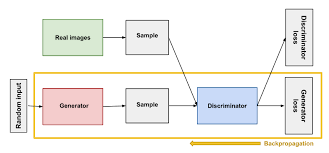
\includegraphics[width=4cm]{figures/1174086/9/4.png}
		\centering
		\caption{Illustrasi Network Generator}
	\end{figure}
	Jelaskan dengan ilustrasi gambar sendiri arsitektur discriminator network dari Age-cGAN.
	\hfill \break


	Tujuan utama dari jaringan diskriminator adalah untuk mengidentifikasi apakah gambar yang disediakan adalah palsu atau nyata. Hal ini dilakukan dengan melewati gambar melalui serangkaian lapisan sampling bawah dan beberapa lapisan klasifikasi. Dengan kata lain, ini memprediksi Apakah gambar itu nyata atau palsu. Seperti jaringan lain, Jaringan diskriminator lain dalam jaringan convolutional. Ini berisi beberapa blok convolutional. Setiap blok convolutional berisi lapisan convolutional, lapisan normalisasi batch, dan fungsi aktivasi, selain blok convolutional pertama, yang tidak memiliki lapisan normalisasi batch. 
		
	\begin{figure}[H]
		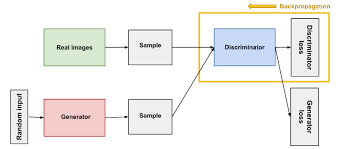
\includegraphics[width=4cm]{figures/1174086/9/5.png}
		\centering
		\caption{Illustrasi Discriminator Network}
	\end{figure}
	\item Jelaskan dengan ilustrasi gambar apa itu pretrained Inception-ResNet-2 Model.
	\hfill \break
	pre-trained Inception-ResNet-2 network, sekali disediakan dengan gambar, mengembalikan yang sesuai embedding. Tertanam yang diekstrak untuk gambar asli dan gambar direkonstruksi dapat dihitung dengan menghitung jarak Euclidean dari yang tertanam.
	\begin{figure}[H]
		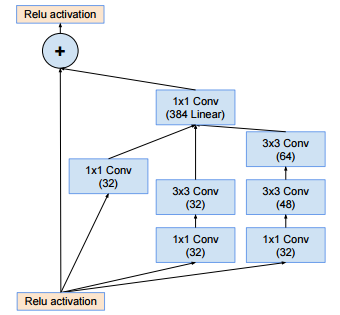
\includegraphics[width=4cm]{figures/1174086/9/6.png}
		\centering
		\caption{Illustrasi Inception-ResNet-2 Model.}
	\end{figure}
	\item Jelaskan dengan ilustrasi gambar sendiri arsitektur Face recognition network Age-cGAN.

	\hfill \break
	Tujuan utama dari jaringan pengenalan wajah adalah untuk mengenali identitas seseorang dalam gambar yang diberikan.
\begin{figure}[H]
		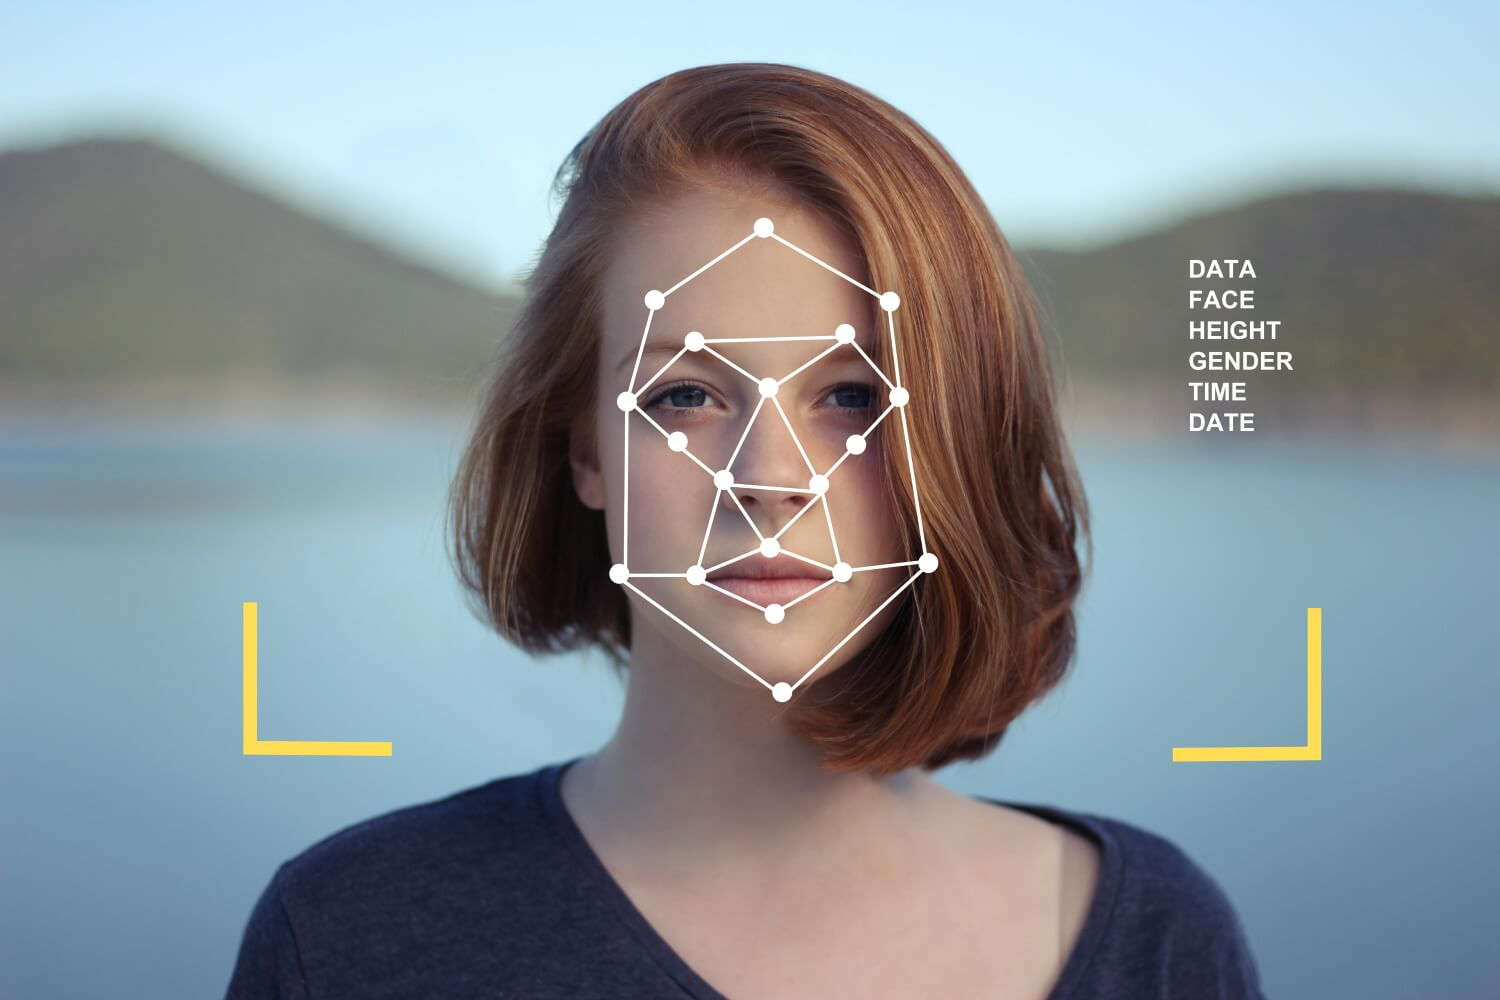
\includegraphics[width=4cm]{figures/1174086/9/7.jpg}
		\centering
		\caption{Illustrasi Face recognition network Age-cGAN.} 
\end{figure}
	\item . Sebutkan dan jelaskan serta di sertai contoh-contoh tahapan dari Age-cGAN

	\hfill \break
	Age-cGAN memiliki beberapa tahapan pelatihan. Seperti disebutkan di bagian sebelumnya, Age-cGAN memiliki empat jaringan, yang dilatih dalam tiga tahap. Pelatihan AgecGAN terdiri dari tiga tahap:

	\begin{itemize} 
			\item pelatihan GAN bersyarat: pada tahap ini, kita melatih jaringan Generator dan jaringan diskriminator.
    		\item awal pendekatan vektor laten: pada tahap ini, kami melatih jaringan Encoder.
    		\item optimasi vektor laten: pada tahap ini, kami mengoptimalkan kedua encoder dan jaringan generator.
		\end{itemize}
	\item Berikan contoh perhitungan fungsi training objektif
	\hfill \break
	


	\item Berikan contoh dengan ilustrasi penjelasan dari Initial latent vector approximation
	\hfill \break
	Perkiraan vektor laten awal adalah metode untuk memperkirakan vektor laten untuk mengoptimalkan rekonstruksi gambar wajah. Untuk memperkirakan vektor laten, kami memiliki jaringan Encoder. Kami melatih jaringan Encoder pada gambar yang dihasilkan dan gambar nyata. Setelah dilatih, Jaringan Encoder akan mulai menghasilkan vektor laten dari Distribusi. Tujuan pelatihan fungsi untuk pelatihan jaringan Encoder adalah kehilangan jarak Euclidean.

	\begin{figure}[H]
		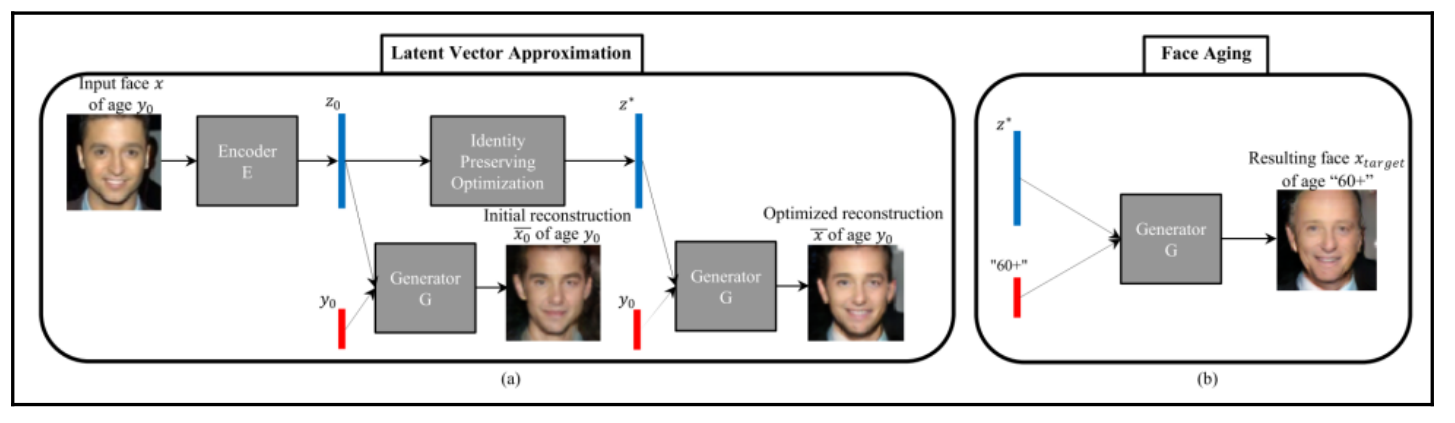
\includegraphics[width=4cm]{figures/1174086/9/8.png}
		\centering
		\caption{Illustrasi Initial latent vector approximation}
	\end{figure}
	\item Berikan contoh perhitungan latent vector optimization
	\hfill \break
	
	\begin{figure}[H]
		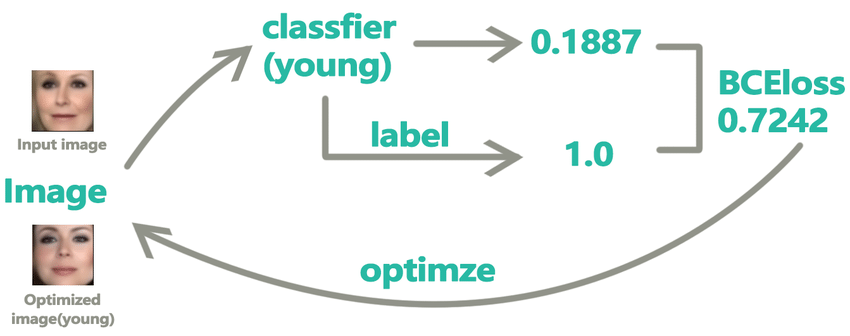
\includegraphics[width=4cm]{figures/1174086/9/9.png}
		\centering
		\caption{Contoh Perhitungan Latent vector optimization}
	\end{figure}

\end{enumerate}
\subsection{Praktek}
\begin{enumerate}
\item Jelaskan bagaimana cara ekstrak file dataset Age-cGAN menggunakan google colab.
Menggunakan Google Colab, dimana membuat notebooks baru, kemudian membuat ekstraksi file dari link dataset.
\lstinputlisting[firstline=1, lastline=4]{src/1174086/9/1174086.py}



\item Jelaskan bagaimana kode program bekerja untuk melakukan load terhadap dataset yang sudah di ekstrak, termasuk bagaimana penjelasan kode program perhitungan usia.
Dibawah ini merupakan code untuk melakukan fungsi perhitungan usia.

\lstinputlisting[firstline=6, lastline=31]{src/1174086/9/1174086.py}

	\item Jelaskan bagaimana kode program The Encoder Network bekerja dijelaskan dengan bahawa awam dengan ilustrasi sederhana.
Proses Encoder berfungsi untuk mempelajari pemetaan terbalik dari gambar wajah dan kondisi usia dengan vector latent Z.

		\lstinputlisting[firstline=33, lastline=73]{src/1174086/9/1174086.py}

	\item Jelaskan bagaimana kode program The Generator Network bekerja dijelaskan dengan bahawa awam dengan ilustrasi sederhana.
Proses Generator agar bekerja dengan baik dibutuhkan representasi dari gambar wajah dan vector kondisi sebagai inputan yang menghasilkan sebuah gambar.

		\lstinputlisting[firstline=75, lastline=104]{src/1174086/9/1174086.py}

        	\item Jelaskan bagaimana kode program The Discriminator Network bekerja dijelaskan dengan bahawa awam dengan ilustrasi sederhana.
Proses Discriminator untuk membedakan antara gambar asli dan gambar palsu.

		\lstinputlisting[firstline=116, lastline=148]{src/1174086/9/1174086.py}

        	\item Jelaskan bagaimana kode program Training cGAN bekerja dijelaskan dengan bahawa awam dengan ilustrasi sederhana.
Proses Training cGAN ini dengan load file .mat pada dataset lalu epoch sebanuak 500 kali.

		\lstinputlisting[firstline=150, lastline=167]{src/1174086/9/1174086.py}

        	\item Jelaskan bagaimana kode program Initial dan latent vector approximation bekerja dijelaskan dengan bahawa awam dengan ilustrasi sederhana.
Initial dan Latent Vector Approximation bekerja melakukan predicsi epoch yang telah di buat sebanyak 500 kali, dan nanti hasilnya ada di folder result.

		\lstinputlisting[firstline=169, lastline=217]{src/1174086/9/1174086.py}
\end{enumerate}

\subsection{Bukti Tidak Plagiat}
\begin{figure}[H]
    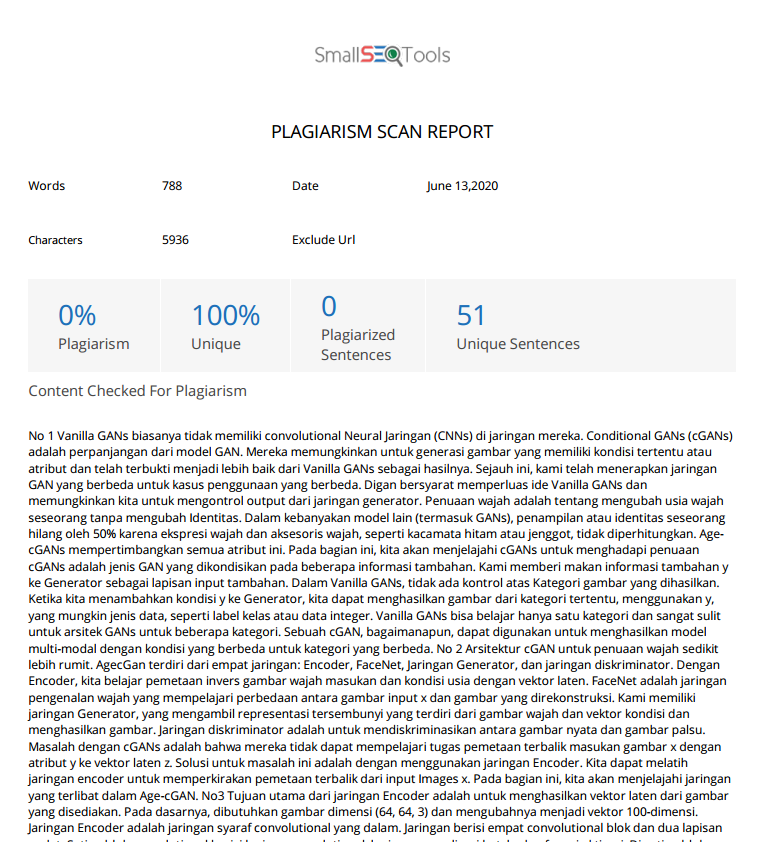
\includegraphics[width=4cm]{figures/1174086/bukti/9.png}
    \centering
    \caption{Tidak Melakukan Plagiat Pada Ch 9}
\end{figure}